%
\documentclass[showpacs, superscriptaddress, showpacs, letterpaper, showkeys,
preprintnumbers, altaffilletter, amssymb, amsmath, amsfonts, prd,
onecolumn, floatfix, nofootinbib]{revtex4-1}

\usepackage{graphics}
\usepackage{color}
\usepackage{leftidx}
\usepackage{multirow}
\usepackage[colorlinks=true]{hyperref}
%\usepackage[caption=false]{subfig}
\usepackage{subcaption}

\def\gw#1{gravitational wave#1 (GW#1)\gdef\gw{GW}}
\newcommand{\gws}{gravitational waves }
\newcommand{\subgw}{_{\textrm{\scriptsize{GW}}}}
\newcommand{\diff}{{\mathrm d}}
\newcommand{\ee}[1]{\!\times\!10^{#1}}
\newcommand{\model}{{\mathcal H}}
\newcommand{\prob}{{\rm Pr}}
\newcommand{\far}{{\mathcal R}_0}
\newcommand{\msun}{{\mathrm M}_{\odot}}

% XXX: not sure why this isn't getting picked up elsewhere but this is a
% workaround for now
\def\mnras{\ref@jnl{MNRAS}}

\def\imbh#1{intermediate mass black hole#1(IMBH#1)\gdef\imbh{IMBH}}
\def\smbh#1{supermassive black hole#1(SMBH#1)\gdef\smbh{SMBH}}
\def\bbh#1{binary black hole#1 (BBH#1)\gdef\bbh{BBH}}
\def\bh#1{black hole#1 (BH#1)\gdef\bh{BH}}
\def\ns#1{neutron star#1 (NS#1)\gdef\ns{NS}}
\def\gw#1{gravitational wave#1 (GW#1)\gdef\gw{GW}}
\def\sn#1{core-collapse supernova#1 (CCSN#1)\gdef\sn{CCSN}}
\def\pnw#1{post-Newtonian#1 (PN#1)\gdef\pnw{PN}}
\def\eos#1{equation of state#1 (EoS#1)\gdef\eos{EoS}}
\def\grb#1{gamma-ray burst#1 (GRB#1)\gdef\grb{GRB}}
\def\amr#1{adaptive mesh refinement#1 (AMR#1)\gdef\amr{AMR}}
\def\isco#1{innermost stable circular orbit#1 (ISCO#1)\gdef\isco{ISCO}}
\def\cwb#1{Coherent WaveBurst#1 (CWB#1)\gdef\cwb{CWB}}

\newcommand{\red}[1]{{\color{red}{#1}}}
\newcommand{\about}[1]{{\color{blue}{[THIS SECTION: #1]}}}
\newcommand{\add}[1]{{\color{magenta}{[TO INCLUDE: #1]}}}
\newcommand{\JC}[1]{{\color{magenta}{[[JC #1]]}}}
\newcommand{\placeholder}[2]{{\color{red}{[PLACEHOLDER](#1):}}{\color{red}{[}}#2{\color{red}{]}}}
\providecommand{\todo}[1]{{\color{red}$\blacksquare$~\textsf{[TODO: #1]}}}


%%%%%% Useful for draft editing
\usepackage{soul} 
\usepackage{ulem} \normalem 
\newcommand{\ec}[1]{{\noindent\color{red}{\it [[#1]] }}}
\newcommand{\laura}[1]{{\color{blue}{#1}}}
\newcommand{\LC}[1]{{\color{red}{[[LC #1]]}}}
\newcommand{\AB}[1]{{\color{blue}{[[AB #1]]}}}
\newcommand{\highlight}[1]{\colorbox{yellow}{#1}}
\newcommand{\simgt}{\mbox{$^{>}_{\sim}$}}
%\newcommand{\simgt}{\stackrel{>}{_{\sim}}} 

\begin{document}

%\title{Inferences From The Post-Merger Gravitational Wave Signal In Binary
%Neutron Star Coalescence}
\title{Towards Bayesian Parameter Estimation For The Post-Merger Gravitational
Wave Signal In Binary Neutron Star Coalescence}

\author{J. Clark}
\affiliation {University of Massachusetts Amherst, Amherst, MA 01003, USA } 
%\author{A. Bauswein}
%\affiliation{Max Planck Institute For Astrophysics}
%\affiliation{Aristotle University of Thessaloniki}
%\author{L. Cadonati}
%\affiliation {University of Massachusetts Amherst, Amherst, MA 01003, USA } 
%\affiliation {Cardiff University, Cardiff, CF24 3AA, United Kingdom }
%\author{H.-T. Janka}
%\affiliation{Max Planck Institute For Astrophysics}
%\author{N. Stergioulas}
%\affiliation{Aristotle University of Thessaloniki}

\date{\today}


\begin{abstract}
Some notes \& preliminary results for Bayesian post-merger analysis.  So far, we
have the ability to compute matches (time- and phase-maximised overlap) between
numerical post-merger signals and a simple template.  This part also estimates
the expected bias in the recovery of $f_2$.  Finally,  we have preliminary
estimates of $f_2$ measurability for optimally oriented signals in a single
detector as a function of distance for the DD2 (1.35+1.35) waveform using a
parallel-tempering MCMC algorithm with the aforementioned templates.  The goal
at this point is to extend these results to a few different waveforms and then
perform a small demonstration of combining the measurements, in a coherent
Bayesian manner, from multiple post-merger signals for a single EOS with
slightly different binary masses.  
\end{abstract}

%   \keywords{}
%
\pacs{
04.80.Nn, % Gravitational wave detectors and experiments
07.05.Kf, % Data analysis: algorithms and implementation; data management
97.60.Jd,  % Neutron stars (see also 26.60.-c Nuclear matter aspects of neutron stars in—Nuclear physics)
04.25.dk % Numerical studies of other relativistic binaries
}

\maketitle
%%%%%%%%%%%%%%%%%%%%%%%%%%%%%%%%%%%%%%%%%%%%%%%%%%%%
% --- INTRODUCTION
\section{Introduction}
%\input{intro.tex}

%%%%%%%%%%%%%%%%%%%%%%%%%%%%%%%%%%%%%%%%%%%%%%%%%%%%
% --- TEMPLATES / WAVEFORM MODEL

% --- Ad hoc Waveform Model
\section{Ad hoc Templates}
From visual inspection of the post-merger waveforms (as well as from more
detailed spectral analysis) one is immediately inclined to suspect that a
simple, monochromatic damped-sinusoid may be sufficient to recover the peak
frequency ($f_2$) using a matched-filter analysis.  However, closer inspection
of the spectral content reveals that the dominant post-merger oscillation peak
is closer to a Gaussian, rather than a Lorentzian.  Furthermore, there is often
a slight asymmetry in the post-merger peak arising from the non-stationarity of
the instantaneous frequency over the evolution of the post-merger remnant.
While it is tempting to try to model the frequency evolution based on numerical
simulations, such a template will necessarily introduce a large number of
parameters, complicating the data analysis.  Here, we will consider the expected
performance of four very simple analytical prescriptions for the post-merger
signal:
\begin{description}
% --- RING DOWN
\item [Exponentially-damped Sinusoid (`Ring-down', RD)]
\begin{equation}\label{eq:ringdown}
h_{RD}(t-t_0) = 
\begin{cases}
A_0 \sin (2\pi f_0 t + \phi_0) e^{-\frac{t}{2\tau}}~\text{for
$t \geq t_0$} \\
0~\text{otherwise.}
\end{cases}
\end{equation}
% --- GAUSS DOWN
\item [Gaussian-damped Sinusoid (`Gauss-down', GD)]
\begin{equation}\label{eq:gaussdown}
h_{GD}(t-t_0) = 
\begin{cases}
A_0 \sin (2\pi f_0 t + \phi_0) e^{-\frac{t^2}{2\tau^2}}~\text{for
$t \geq t_0$} \\
0~\text{otherwise.}
\end{cases}
\end{equation}
% --- RING CHIRP
\item [Exponentially-damped Chirp (`Chirping Ring-down', CRD)]
We now allow the phase of the sinusoidal part of the waveform to evolve
such that the frequency increases linearly in time:
\begin{equation}\label{eq:ringchirp}
h_{RC}(t-t_0) = 
\begin{cases}
A_0 \sin (2\pi f_0 t + \phi(t) + \phi_0) e^{-\frac{t}{2\tau}}~\text{for
$t \geq t_0$} \\
0~\text{otherwise,}
\end{cases}
\end{equation}
where the phase evolution is given by,
\begin{equation}\label{eq:phase_evol}
\phi(t) = \text{Look this up \dots}.
\end{equation}
% --- GAUSS CHIRP
\item [Gaussian-damped Chirp (`Chirping Gauss-down', CGD)]
We now allow the phase of the sinusoidal part of the waveform to evolve
linearly in time:
\begin{equation}\label{eq:gausschirp}
h_{GC}(t-t_0) = 
\begin{cases}
A_0 \sin (2\pi f_0 t + \phi(t) + \phi_0) e^{-\frac{t^2}{2\tau^2}}~\text{for
$t \geq t_0$} \\
0~\text{otherwise,}
\end{cases}
\end{equation}
where the phase evolution is again given by equation~\ref{eq:phase_evol}.
\end{description}
%
In the case of the ring-down and the Gauss-down, the center frequency $f_0$ is
our estimator for $f_2$ (i.e., the post-merger peak frequency of interest).  For
the chirping signals, our estimator for $f_2$ is based on the \emph{average}
frequency content of the damped-chirp (the section below will elucidate this
point). In the current code-setup, we are able to recover the joint posterior
probability density function on the initial frequency and the total change in
frequency over the full duration of the waveform.  I still need to make sure I
understand how to get to the desired estimator for $f_2$ from these measured
parameters.

% --- Match and bias for different waveforms
\subsection{Expected Template Performance: Match \& Frequency Bias}
Our predictions of templates' relative performance are based on the match; the
overlap $\sigma$ between a numerical waveform $d(t)$ and the template $h(t)$,
maximised over all waveform parameters:
%
\begin{equation}\label{eq:overlap}
\sigma = \frac{(d|h)}{\sqrt{(h|h).(d|d)}},
\end{equation}
%
where the inner product $(a|b)$ is defined:
%
\begin{equation}\label{eq:inner_product}
(a|b) = \int_{f_{\text{min}}}^{f_{\text{max}}}
\frac{\tilde{a}(f)\tilde{b}^*(f)}{S(f)}~\diff f.
\end{equation}
%
Note the explicit presence of the frequency range used for the overlap
calculation.  Our principle interest is in measuring the dominant post-merger
oscillation.  We will, therefore, consider the `broad-band' match over
$[1,~5]$\,kHz which tells us how much of the total SNR in the signal we obtain
with no knowledge of exactly where $f_2$ lies.  Then, when we have found the
frequency which yields the maximum overlap, we will restrict the match
calculation to a narrow range around that frequency in order to determine how
much SNR we can accumulate from that dominant oscillation using our simple
templates.

Finally, we also study the expected bias in the frequency recovery using these
tempates for a variety of post-merger signals.  For the stationary-frequency
waveforms (ring-down and gauss-down) we define the  bias as,
\begin{equation}\label{eq:stationary_bias}
\text{bias} = f_2 - f_0.
\end{equation}
%
For simplicity, I will just define the bias for the chirping waveforms as,
\begin{equation}\label{eq:chirp_bias}
\text{bias} = f_2 - f_p,
\end{equation}
%
where $f_p$ is the frequency of the peak of the power spectrum of the chirping
waveforms.  I still need to check how to get to $f_p$ from the parameters of the
chirping waveforms (critical for the Bayesian implementation later).  This
approach should work fine for studying the performance of our templates.

\begin{table}
\centering
\begin{tabular}{l | cccc | cccc | cccc}
\toprule
\multirow{2}{*}{Waveform} & \multicolumn{4}{c|}{Max Broadband Match} &
\multicolumn{4}{c|}{Max Narrow-band Match} & \multicolumn{4}{c}{Bias [Hz]} \\
& RD & GD & CRD & CSG & RD & GD & CRD & CGD & RD & GD & CRD & CGD \\
\colrule
APR & 0.254 & 0.252 & 0.271 & 0.268 & 0.899 & 0.916 & 0.983 & 0.986 & 20.18 & 24.18 & 16.18 & 12.18 \\
DD2 & 0.558 & 0.559 & 0.561 & 0.560 & 0.991 & 0.991 & 0.990 & 0.998 & 5.08 & 5.08 & -6.92 &  -0.92 \\
DD2$_{3.3}$ & 0.273 & 0.273 & 0.273 & 0.273 & 0.959 & 0.967 & 0.996 & 0.996 & -7.36 & -9.36 & -5.36 &  -15.36 \\
NL3 & 0.605 & 0.605 & 0.643 & 0.637 & 0.923 & 0.938 & 0.993 & 0.997 & -11.06 & -11.06 & -3.06 & -3.06\\
NL3$_{3.8}$ & 0.399 & 0.406 & 0.447 & 0.445 & 0.891 & 0.913 & 0.971 & 0.986 & -22.93 & -22.93 & -20.93 &  -16.93 \\
SFHo & 0.320 & 0.316 & 0.323 & 0.312 & 0.955 & 0.972 & 0.999 & 0.999 & 6.40 & 8.40 & -11.60 & -3.60 \\
SFHx & 0.430 & 0.426 & 0.431 & 0.426 & 0.967 & 0.977 & 0.995 & 1.000 & 2.23 & 2.23 & -3.78 & 0.232\\
Shen & 0.545 & 0.546 & 0.589 & 0.587 & 0.890 & 0.914 & 0.989 & 0.993 & -21.47 & -19.47 & -15.47 &  -13.47 \\
TM1  & 0.521 & 0.517 & 0.540 & 0.534 & 0.938 & 0.952 & 0.998 & 0.999 & -10.87 & -10.88 & -0.88 & -2.88 \\
TMa  & 0.561 & 0.559 & 0.574 & 0.569 & 0.959 & 0.973 & 0.999 & 1.000 & -13.09 & -13.09 & 0.90 & -3.10 \\
\colrule
\end{tabular}
\caption{Maximal matches and expected frequency biases for numerical waveforms
with the templates described above.  The biases seem surprisingly large and
merit further investigation.  Broadband: match is computed for
$f\in[1,~5]$\,kHz, narrow-band: $f\in[f_0-0.15,~f_0+0.15]$\,kHz, where $f_0$ is
that which yields the maximum match in the broad frequency band.}
\end{table}


%%%%%%%%%%%%%%%%%%%%%%%%%%%%%%%%%%%%%%%%%%%%%%%%%%%%
% --- IMPLEMENTATION IN A SIMPLE ANALYSIS
\section{Implementation With Bayesian Parameter Estimation}
We now have a prototype code in place which will perform a parallel-tempering
MCMC using any of the waveforms described in the previous section.  So far, I
have only produced preliminary resuls for the DD2 waveform, using the Gauss-down
templates.  The algorithm takes a few hours to run on a single injection, but I
believe this can be improved enormously with some more careful tuning of the
MCMC parameters (e.g., burn-in time, number of `walkers', number of samples).

The output are samples from the joint-posterior PDF on the waveform parameters
$\vec{\theta} = (A_0,~f_0,~t_0,~\tau,~\phi_0)$.  For now, at least, we will only
study the marginal posterior on $f_0$:  
\begin{equation}\label{eq:freq_posterior}
p(f_0|D) = \int_{\Psi} p(f_0, \vec{\psi}|M)
p(D|f_0,\vec{\psi},M)~\diff\vec{\psi},
\end{equation}
%
where $\vec{\phi} = (A,~t_0,~\tau,~\phi_0)$.  Again, please note that we are
assuming an optimally oriented source and that we know the orientation with
respect to the detector.  The parameter space of the analysis will increase
significantly if we use multiple detectors and relax that
constraint\footnote{for a single-detector analysis, of course, all of the
extrinsic sky-parameters are degenerate with the overall amplitude scale $A$}.

Note that we place a Gaussian prior with $\sigma=10$\,ms on
the start time of the signal, taken to be the peak-time of the inspiral.  Note
also that we let the MCMC search for $f_0 \in [1.5,~4]$\,kHz and a data
bandwidth of $[1,~5]$\,kHz, to accommodate the finite extent of signals with
$f_0$ at the boundaries.   Again, this is somewhat wider to what we had before
and we can easily restrict it.  It's just interesting to study the most
conservative range possible to begin with.

A particularly useful feature of parallel tempering, in addition to robustly
sampling the posterior, is the computation of the Bayesian \emph{evidence} or
global likelihood of a model $M$,
\begin{equation}\label{eq:evidence}
p(D|M) = \int_{\Theta} p(\vec{\theta}|M)p(D|\vec{\theta}, M)~\diff \vec{\theta}.
\end{equation}
%
We can then form the posterior odds ratio for a signal model $S$ versus a noise
model $N$:
\begin{equation}\label{eq:odds}
\mathcal{O}_{S,N} = \frac{p(S|D)}{p(N|D)} =
\frac{p(S)}{p(N)}\frac{p(D|S)}{p(D|N)}.
\end{equation}
%
which tells us the relative probability of signal vs noise.  While our principle
concern here is the measurement of $f_2$, as opposed to detection at some level
of confidence, we shall see that the posterior odds can be used to increase the
robustness of the frequency estimation.   Finally, it's common to set the prior
odds (the first term in equation~\ref{eq:odds}) to unity, which leaves us with
the evidence ratio or \emph{Bayes factor}:
\begin{equation}\label{eq:bfac}
B_{S,N} = \frac{p(D|S)}{p(D|N)}.
\end{equation}


\subsection{Frequency Recovery}
Figure~\ref{fig:freq_pdf_surfs} shows ensembles of the measured frequency
posterior $p(f_0|D)$ measured at 5, 10, 15 and 20\,Mpc.  Everything behaves
exactly as we'd like it to and, indeed, we do appear \emph{capable of
identifying the correct frequency out to 20\,Mpc}.  Averaging over the sky, and
assuming a 3-detector network with optimal combination of data streams (which is
trivial in this framework), this is a sky-averaged distance of ~15\,Mpc.  The
figures which follow attempt to quantify these results.

\begin{figure}
%\centering
\begin{subfigure}{.4\textwidth}
{\scalebox{0.35}{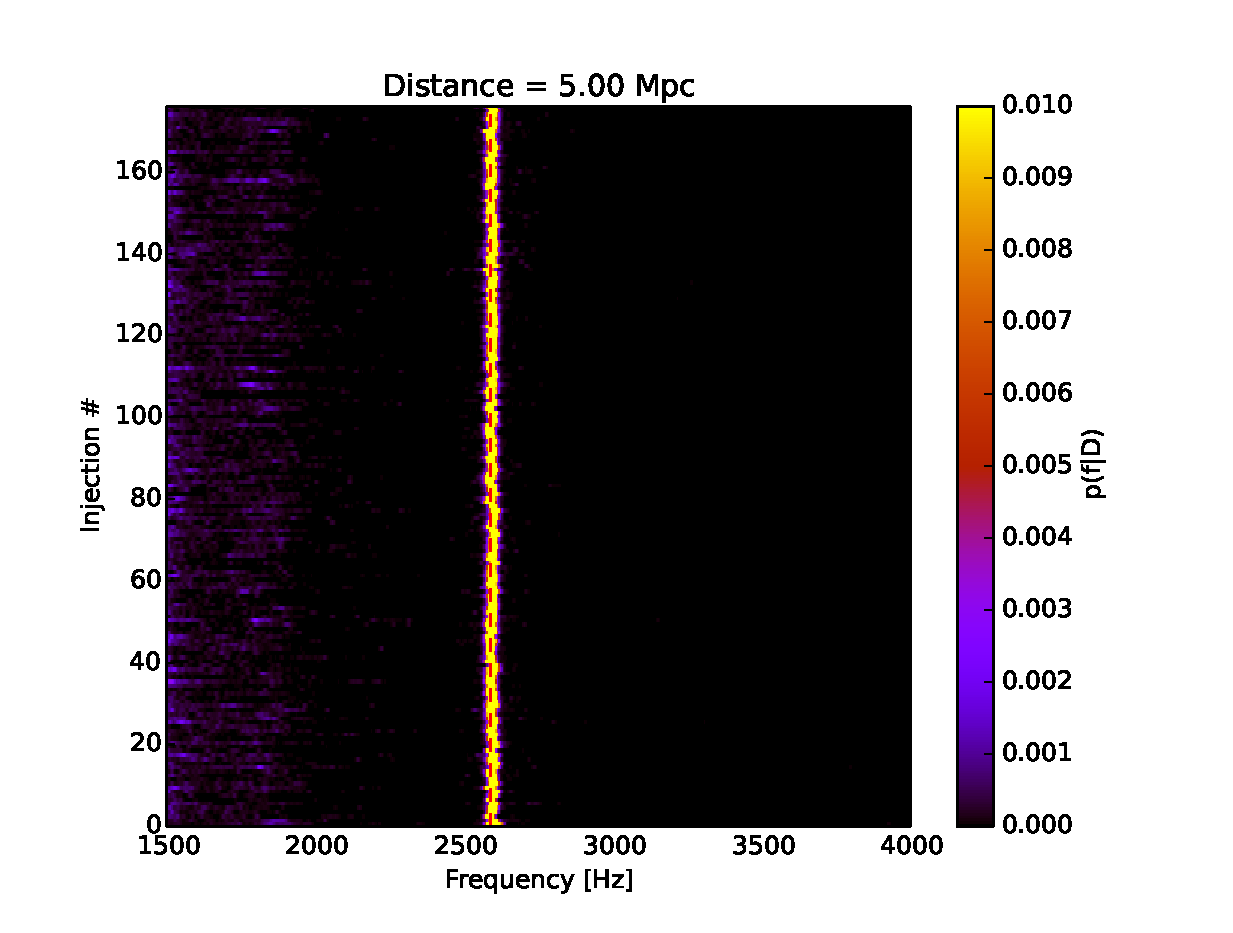
\includegraphics{freqpdfs_dist-5.00.eps}}\label{fig:freqpdfs5Mpc}}
\end{subfigure}
%
\begin{subfigure}{.4\textwidth}
{\scalebox{0.35}{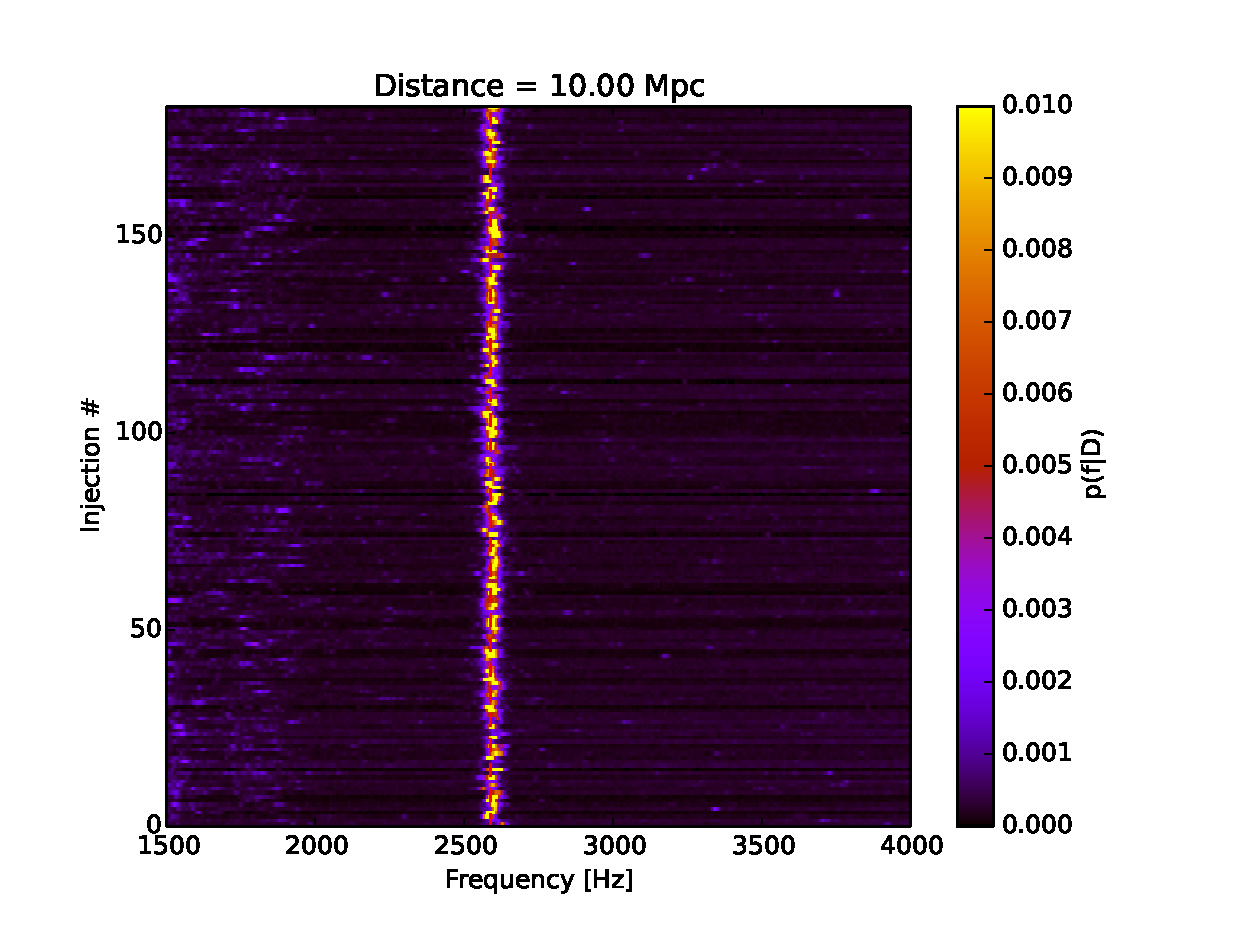
\includegraphics{freqpdfs_dist-10.00.eps}}\label{fig:freqpdfs10Mpc}} 
\end{subfigure}
%                                                
\begin{subfigure}{.4\textwidth}
{\scalebox{0.35}{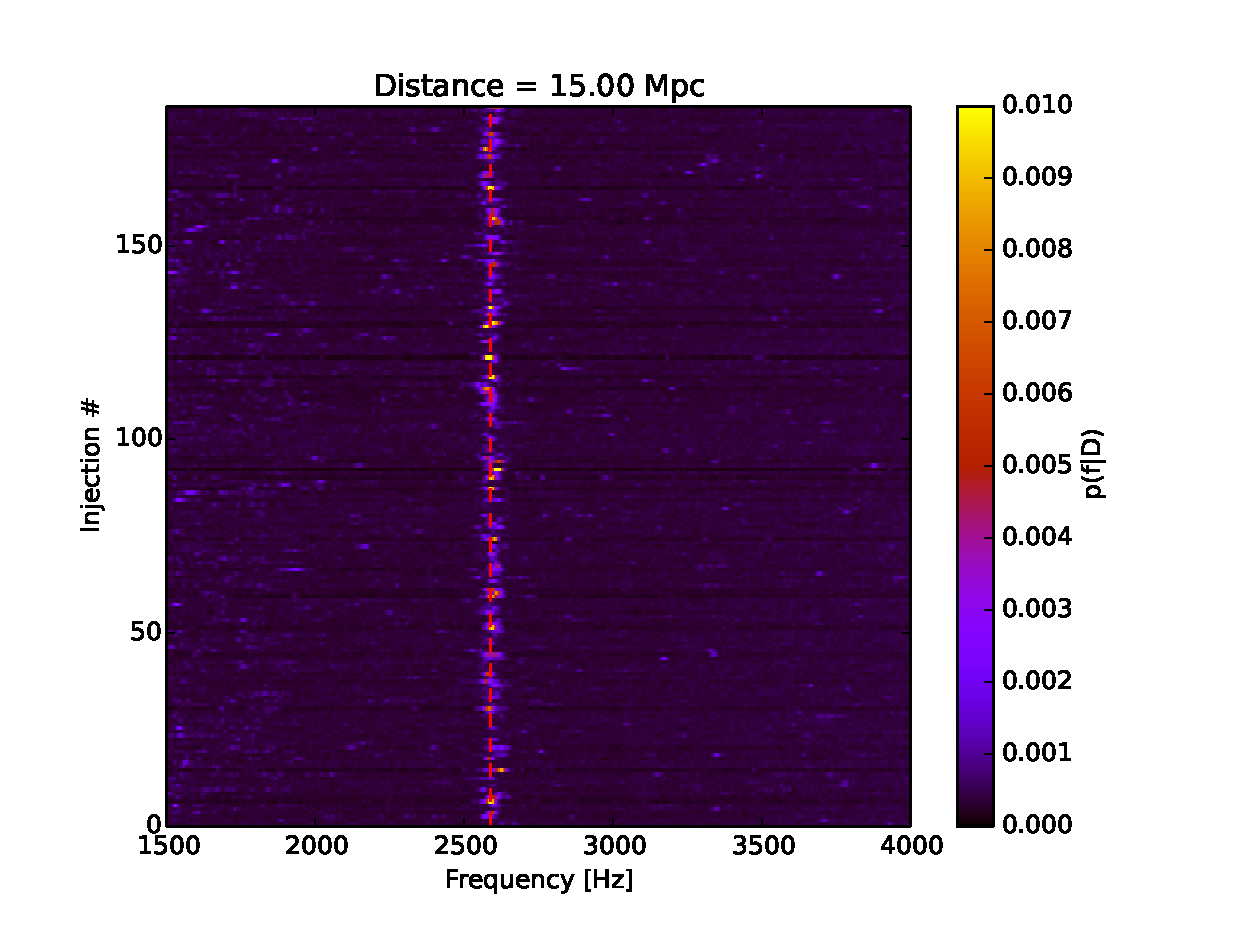
\includegraphics{freqpdfs_dist-15.00.eps}}\label{fig:freqpdfs15Mpc}}
\end{subfigure}
%                                               % 
\begin{subfigure}{.4\textwidth}
{\scalebox{0.35}{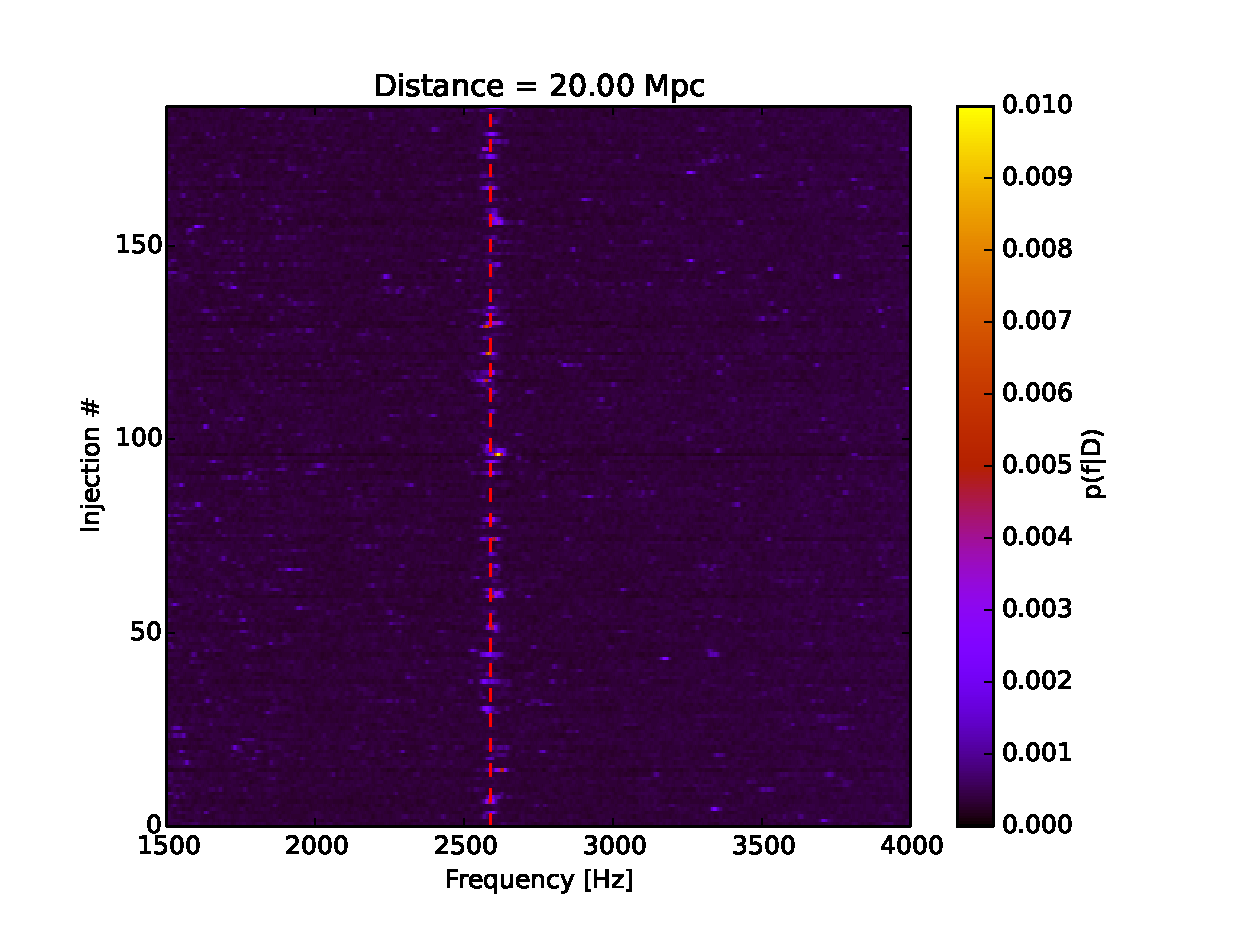
\includegraphics{freqpdfs_dist-20.00.eps}}\label{fig:freqpdfs20Mpc}}
\end{subfigure}
\caption{Frequency posterior PDFs using a single detector for optimally oriented
injections at 5, 10, 15 and 20\,Mpc.  The $y$-axis, `injection number',
corresponds to a different noise realisation in each case.  These are all from
the DD2 EOS.  For nearby injections, the posteriors are sharply peaked (bright
yellow) around the $f_2$ for DD2 (zoom in to see a red dashed line indicating
$f_2$), and zero away from the peak (black surface).  Quieter injections produce
a nearly uniform frequency posterior (purple surface) with a small, but
well-defined peak at the desired value (pink to yellow blobs, embedded in the
purple background).  Note that the louder signals also pick up some probability
from the lower-frequency content.  In our last paper, we placed lower bounds
on $f_2$ which would restrict our prior well above this region.  Here, I'm just
being conservative and I'm curious to see what happens if we search for
$f_2\in[1.5,~4]$\,kHz.\label{fig:freq_pdf_surfs}}
\end{figure}


\begin{figure}
\begin{subfigure}{0.45\textwidth}
{\scalebox{0.4}{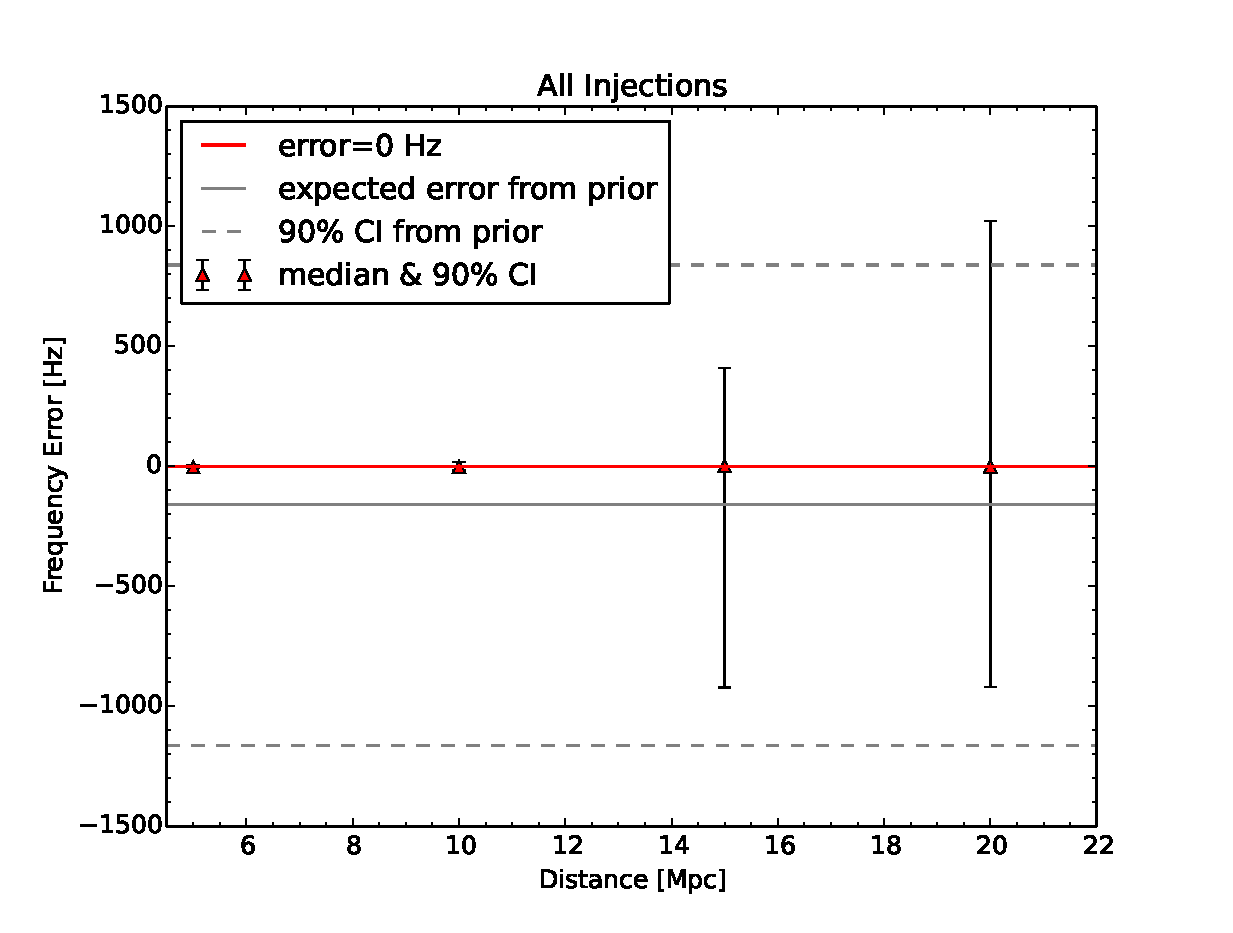
\includegraphics{freqerr.eps}}}
\caption{Box-plot of the error in the estimated frequency using the Gauss-down
template and taking the maximum of the marginal posterior on frequency as the
point estimate.  The boxes show the interquartile range, the red lines in the
boxes are the median values and the whiskers show 1.5$\times$ the interquartile
range.  For reference, we also show as red horizontal lines the result one would
expect to get by `guessing': this is the result we should expect if we made no
measurement at all and simply estimated the peak frequency from our prior; the
solid horizontal red line is the median value of the frequency prior and the
dashed horizontal red lines show the interquartile range.  We therefore confirm
that the measurement of the sources at 20\,Mpc are indeed significantly better
than simply guessing.\label{fig:freqerr}}
\end{subfigure}
\begin{subfigure}{0.45\textwidth}
{\scalebox{0.4}{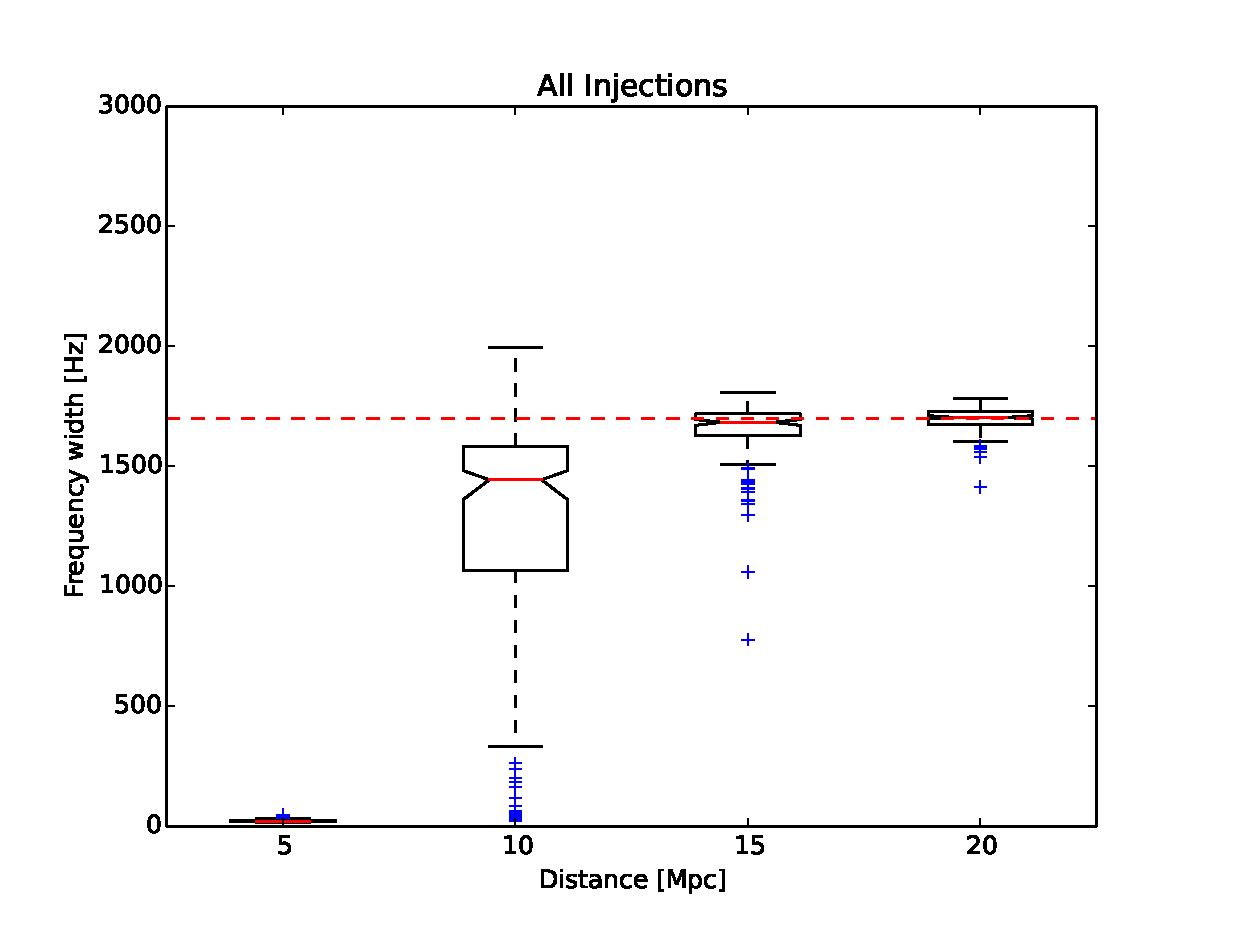
\includegraphics{freqwidth.eps}}}
\caption{Box-plot of the 68\% confidence interval about the maximum of the
frequency using the Gauss-down template and taking the maximum of the marginal
posterior on frequency as the point estimate.  Symbols have the same meaning as
before.  We now see that the confidence interval for the frequency estimate is
extremely wide for quiet signals (as expected) and consistent with the
uncertainty in the measurement one would get from `guessing'.  This does
\emph{not} mean we cannot measure the peak frequency at large distance; it
simply means that the uncertainty in the measurement is large but we can have
some confidence in its \emph{accuracy} from the first panel.\label{fig:freqwidth}\\~\\~\\}
\end{subfigure}
\caption{Frequency recovery assuming signal is present.\label{fig:freqrecovery}}
\end{figure}

\begin{figure}
\begin{subfigure}{0.45\textwidth}
{\scalebox{0.4}{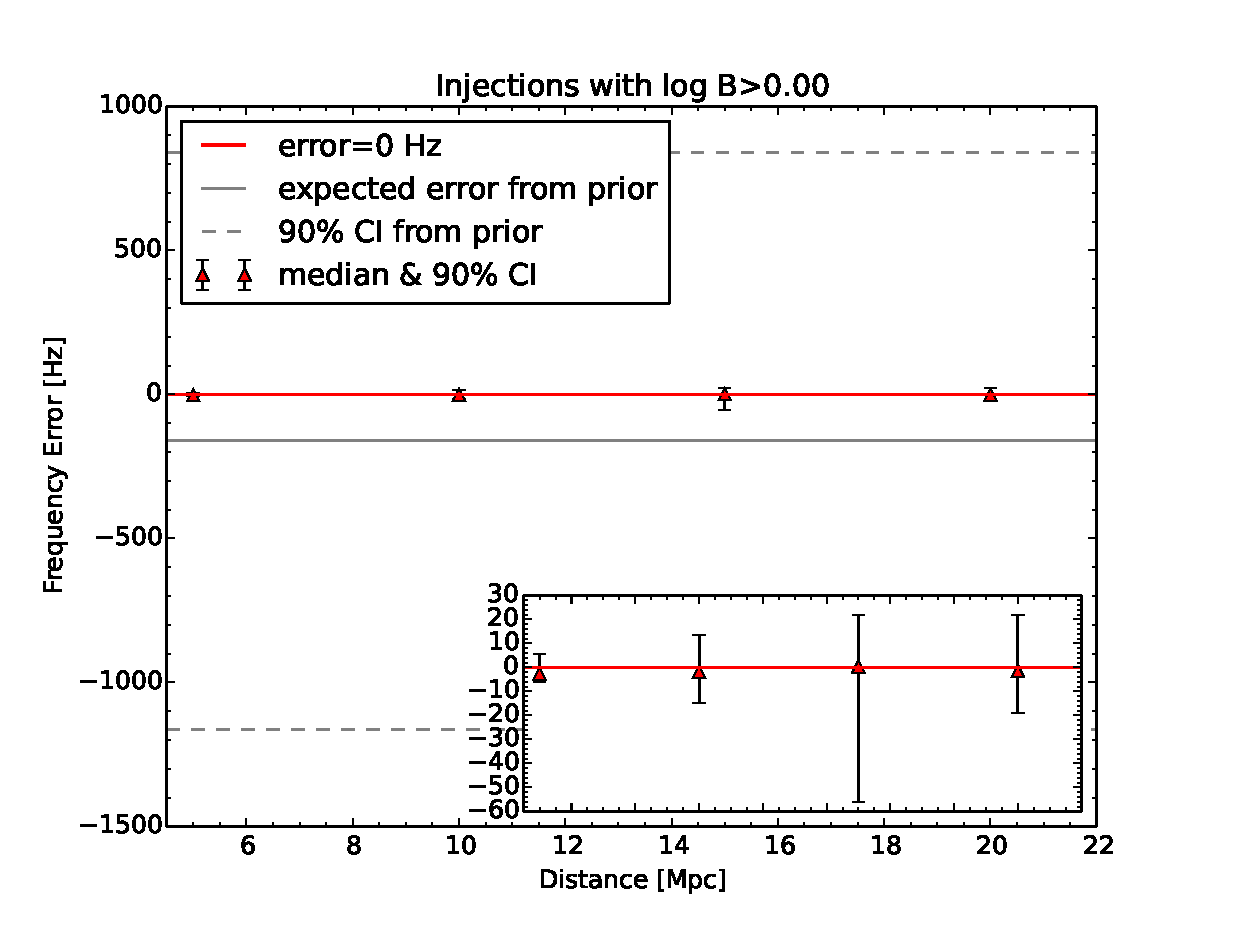
\includegraphics{freqerr_logB-0.00.eps}}}
\caption{As figure~\ref{fig:freqerr} but with the constraint that the posterior
odds ratio (Bayes factor) is greater than unity (i.e., there's a better than
50/50 chance there's a signal there).  We see that this dramatically improves
the accuracy of the frequency measurement.~\\~\\~\\~\\~\\~\\}
\end{subfigure}
\begin{subfigure}{0.45\textwidth}
{\scalebox{0.4}{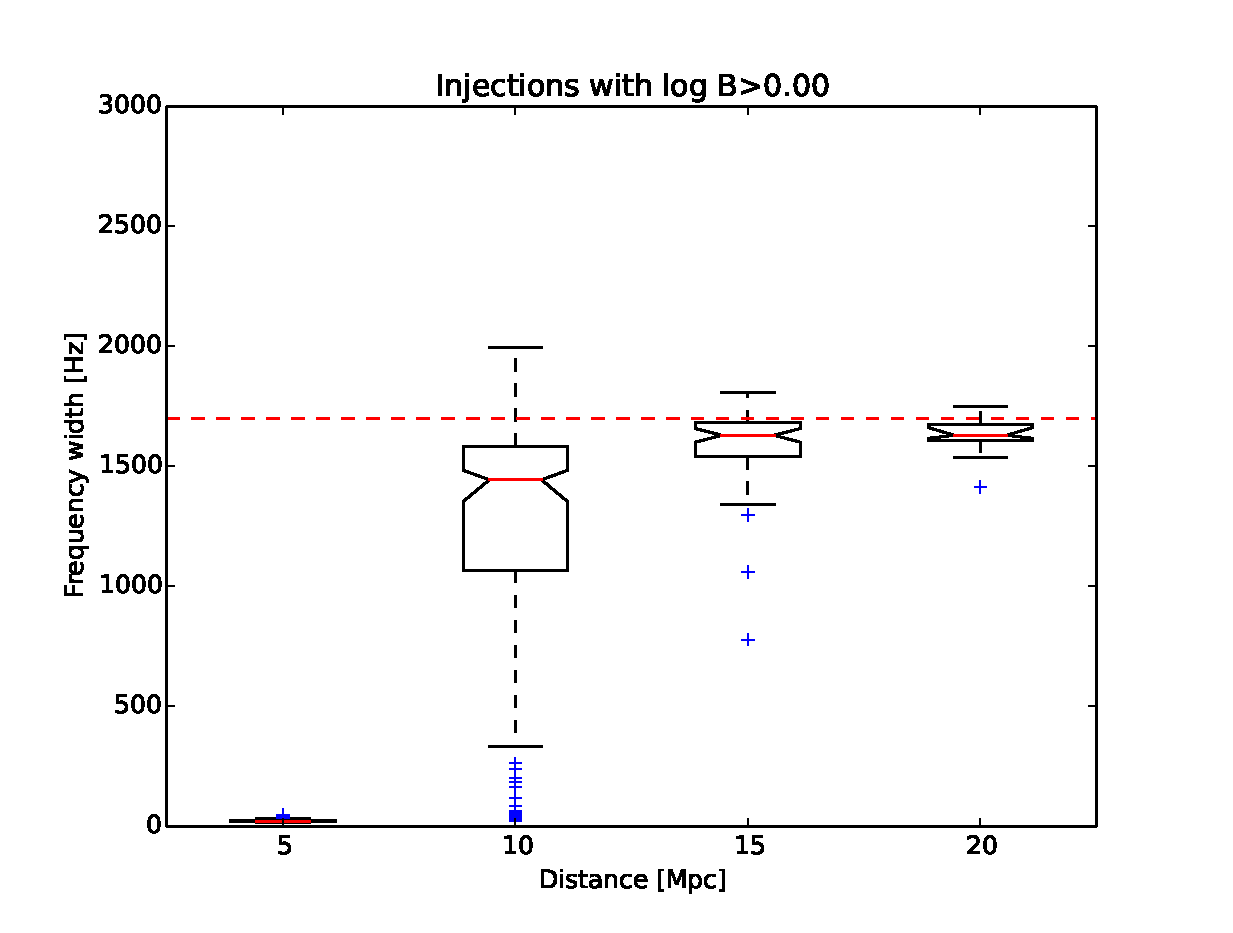
\includegraphics{freqwidth_logB-0.00.eps}}}
\caption{Again, as figure~\ref{fig:freqwidth} with the constraint that $\log
B_{S,N}>0$ (better than 50/50 odds of signal vs noise).  This time, we see
remarkably little change from the previous figure with no constraint.  Given
that the point estimate of the frequency at large distance with the constraint
is so closely clustered around zero error, it is surprising that the posterior
width is so large.  This may point to a trivial code bug or problems in the
kernel density estimation used to smooth the posteriors - I don't yet believe
this result.}
\end{subfigure}
\caption{Frequency recovery with the constraint that there is a better than
50/50 chance we think there's a signal there.\label{fig:constrained_freqrecovery}}
\end{figure}

\begin{figure}
\begin{subfigure}{0.45\textwidth}
{\scalebox{0.4}{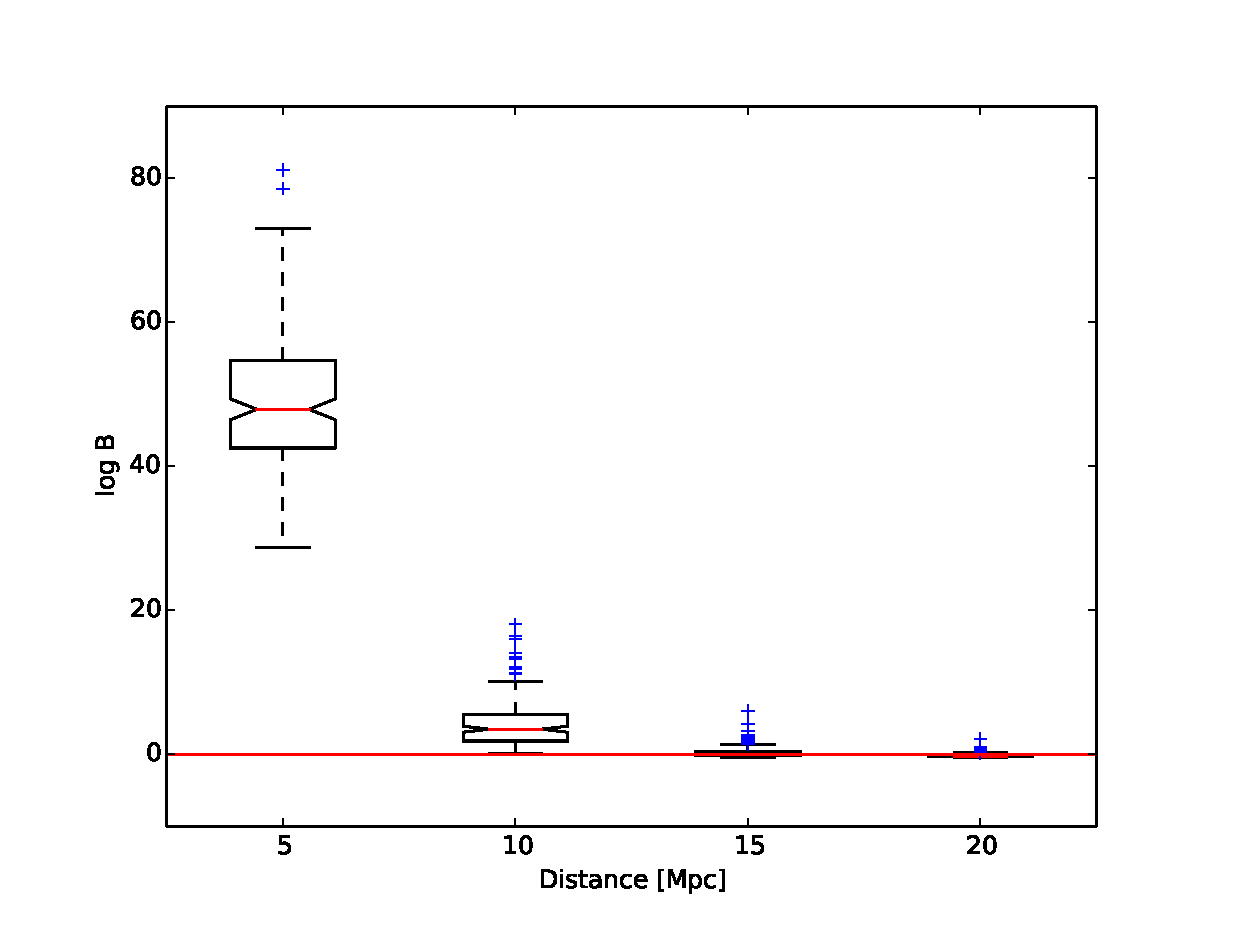
\includegraphics{bayes-boxes.eps}}}
\caption{The distribution of Bayes factors at different distances.  By 20\,Mpc
there is little evidence for the presence of a signal and we basically have to
get lucky.~\\~\\~\\~\\~\\~\\}
\end{subfigure}
\begin{subfigure}{0.45\textwidth}
{\scalebox{0.4}{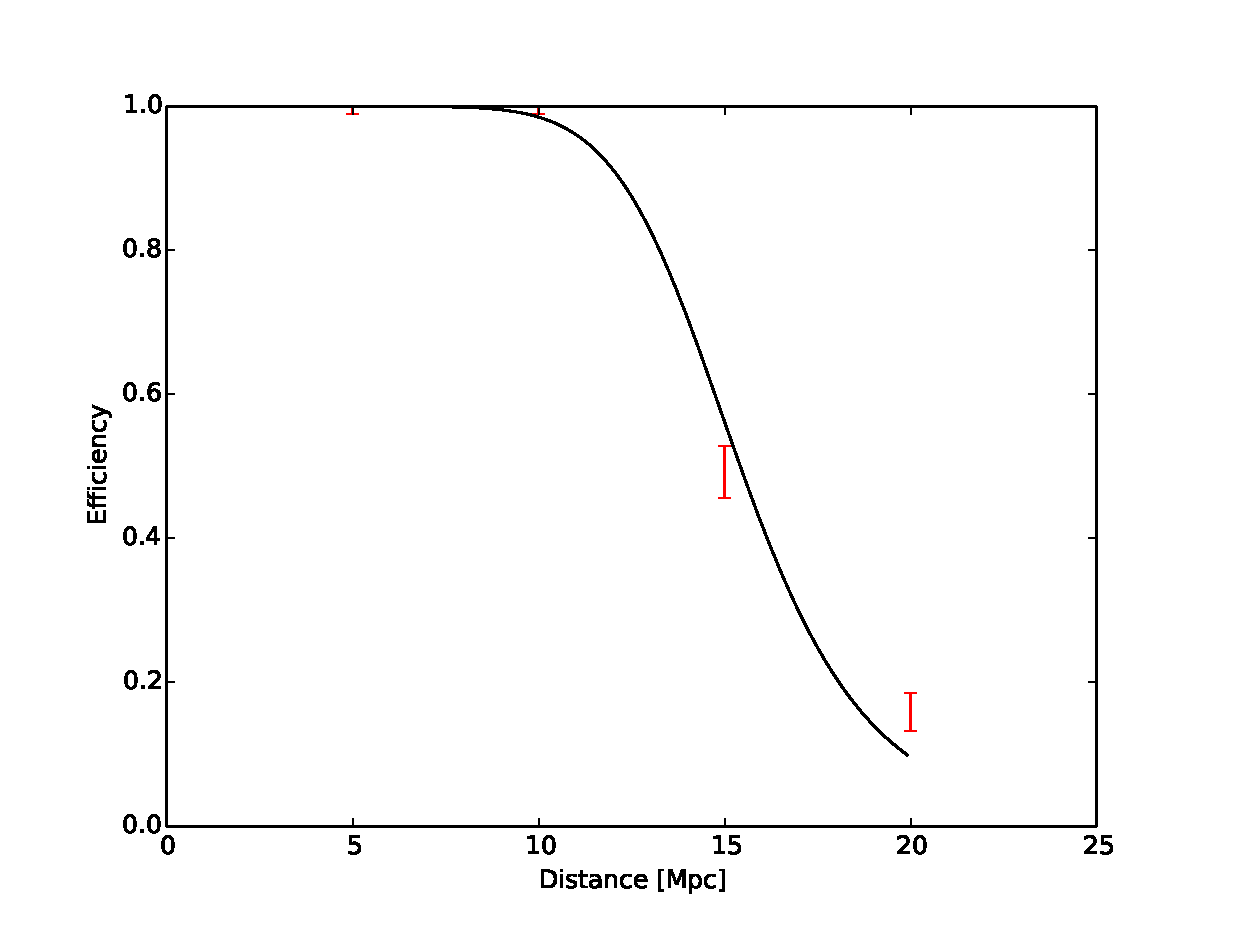
\includegraphics{efficiency_logB-0.00.eps}}}
\caption{The `efficiency' (fraction of signals which produce $\log B_{S,N}>0$ as
a function of distance.  The black curve is a sigmoid fit.  More data is clearly
needed, but we can see that by 20\,Mpc, only about 18\% of signals produce
any evidence for their presence.  However, as we have seen, those 18\% do seem
to have very accurate (if seemingly uncertain) frequency measurements.}
\end{subfigure}
\caption{Behavior of and impact of the Bayes factor constraint $\log B_{S,N}>0$.}
\end{figure}

\end{document}



